\renewcommand{\thechapter}{\roman{chapter}}
\setcounter{chapter}{2}
\setcounter{figure}{0}

\unchapter{Préambule contexte}
\label{chap:preamble_context}

Ce travail va s'inscrire dans une démarche d'aide au diagnostic des lésions de la peau et particulièrement des pathologies de \glsfirst{lm} et \glsfirst{lmm}. De nombreux travaux se sont portés sur l'aide à la détection par ordinateur de lésions de la peau similaires, à l'aide de modalités unique d'imagerie. Néanmoins, peu d'entre eux s'intéressent à une démarche multimodale de cette thématique, soit par non considération de cette application, soit par un manque suffisant de données à leur disposition.\par

La matière première mise à notre disposition permettra une orientation de nos travaux dans le sens de la multimodalité. En effet, l'une des problématique majeure aujourd'hui en dermatologie, est ce que les médecins qualifient de zone d'indécision, également appelée \textit{zone grise}. Il s'agit d'une catégorie de cas cliniques pour lesquels le médecin n'a pas à un instant $t$ suffisamment d'information en sa possession ou les connaissances suffisantes pour prendre une décision. Ces cas nécessitent souvent une prise en charge plus importante, avec l'aide d'autres spécialistes ou encore avec notamment de nouveaux examens plus spécifiques.\par

Nous souhaitons par ce travail, amener diverses techniques et outils permettant une aide à la décision dans la gestion de cette zone grise, et ainsi améliorer la condition clinique en service de dermatologie. Ainsi, nous proposons un schéma macroscopique de cet objectif en \Cref{fig:scheme_reduce_indecision}.\par

\begin{figure}[H]
    \centering
    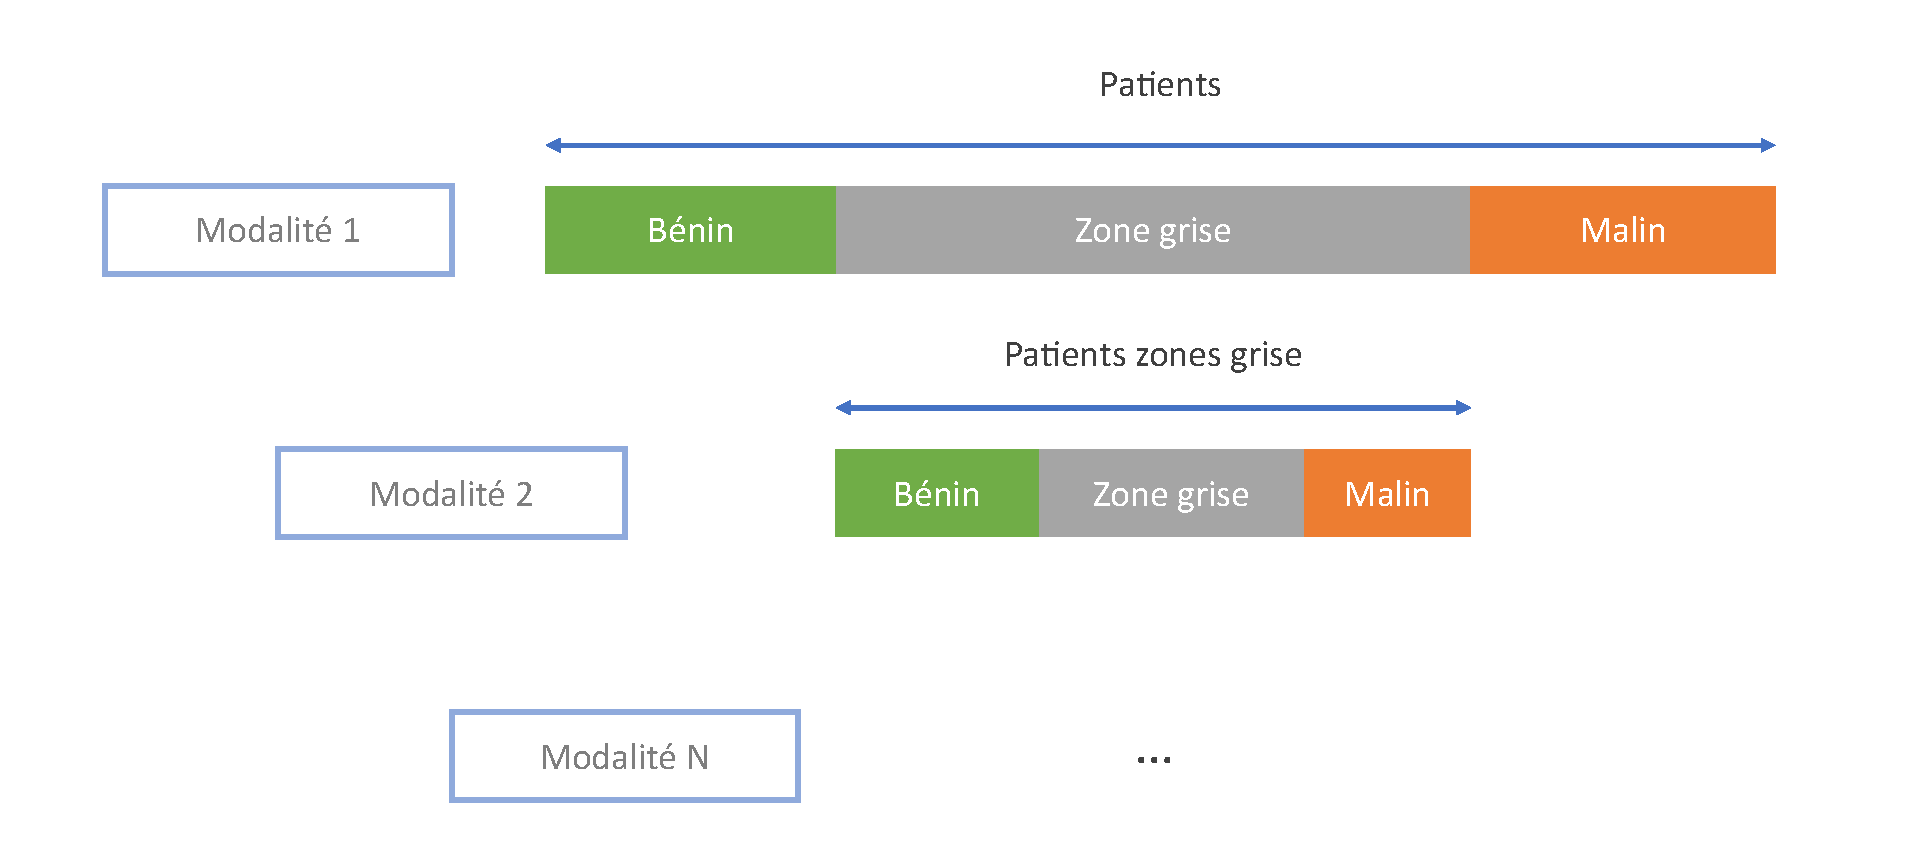
\includegraphics[width=\linewidth]{contents/ii_preamble_context/resources/scheme_reduce_indecision.pdf}
    \caption{Représentation du processus de réduction de l'indécision du médecin ou \textit{zone grise}. Ainsi, ce travail à pour objectif de réduire par l'apport de nouvelles modalités les divers cas portant à confusion de manière similaire au processus congnitif des dermatologues.}
    \label{fig:scheme_reduce_indecision}
\end{figure}\par

A cette fin, nous mobiliserons des connaissances en provenance propre à la peau, aux modalités d'observation et à l'intelligence artificielle, tel que représenté en \Cref{fig:scheme_our_work}. Pour cela, nous mettrons à disposition du lecteur l'ensemble des bases nécessaire à la compréhension de ce sujet au travers de cette partie de contexte. Nous débuterons au sein du \Cref{chap:chapter_1} par une présentation de la peau, c'est à dire l'organe majeure de cette étude. Puis, nous procéderons à l'aide du \Cref{chap:chapter_2} à une mise en évidence des principes d'interaction entre la peau et la lumière, avant de présenter les techniques de visualisations mises à disposition des médecins. Pour finir cette partie, nous réaliserons un descriptif des méthodes d'intelligence artificielle applicable à ce travail.\par

\begin{figure}[H]
    \centering
    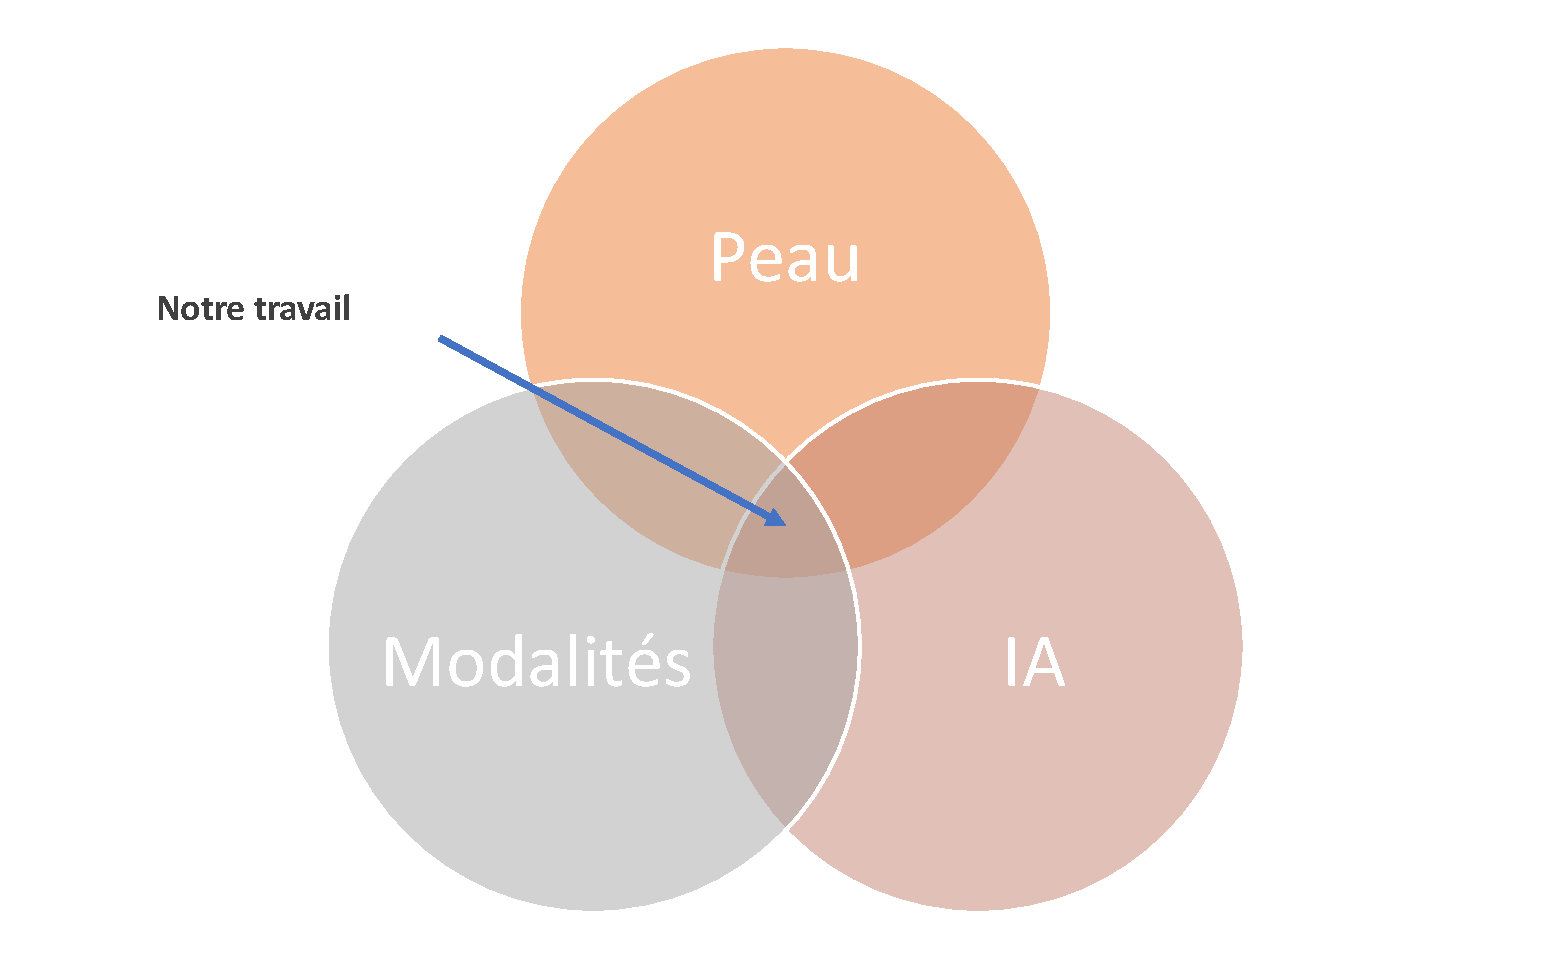
\includegraphics[width=\linewidth]{contents/ii_preamble_context/resources/scheme_our_work.pdf}
    \caption{Macro représentation des domaines impliqués de cette thématique de recherche. Notre travail se retrouve ainsi au confluents de connaissance de la peau, des modalités d'imagerie permettant son acquisition et des domaines de l'intelligence artificielle.}
    \label{fig:scheme_our_work}
\end{figure}\par